\section{Literature Review}

\subsection{Types of Machine Learning Methods}
\begin{itemize}
    \item compare supervised vs unsupervised learning
    \item supervised learning will be used for land zone segmentation and vegetation analysis
    \item unsupervised learning might be used for dimensionality reduction
    \item this chapter only makes sense if unsupervised learning is put to good use
\end{itemize}

\subsection{Convolutional Neural Networks}
One subclass of neural networks is called Convolutional Neural Network (CNN) ~\cite[p.~359]{praxiseinstieg_ml17}. These types of networks show great results on data with a grid-like topology. Thus, they are often used for processing of image or video data. In traditional neural networks the layers are often densely connected, meaning every neuron of one layer is connected to every neuron in the next layer. For grid-like data this is not very efficient, because cells close to each other are often more likely to be correlated. Instead of dense connections, CNNs use operations called \emph{convolution} and \emph{pooling}, which allow to take spatial properties of input data into account. The following sections explain the commonly used operations in CNNs.

\subsubsection{Convolution}
Convolution is a mathematical operation that uses weighted point-by-point multiplication of two matrices resulting in a scalar value. The concept is shown in figure~\ref{fig:convolution}. The notation $n_{k, i, j}$ represents a neuron at row $i$ and column $j$ in layer $k$. For a convolutional layer, neuron $n_{k, i, j}$ is connected to all neurons $n_{k-1, i, j}$ to $n_{k-1, i + f_w -1, j + f_h -1}$. The neurons in layer $k-1$ are therefore called receptive field of $n_{k, i, j}$ with a kernel width of $f_w$ and kernel height of $f_h$.~\cite[p.~361f]{praxiseinstieg_ml17}

\begin{figure}[h]
    \centering
    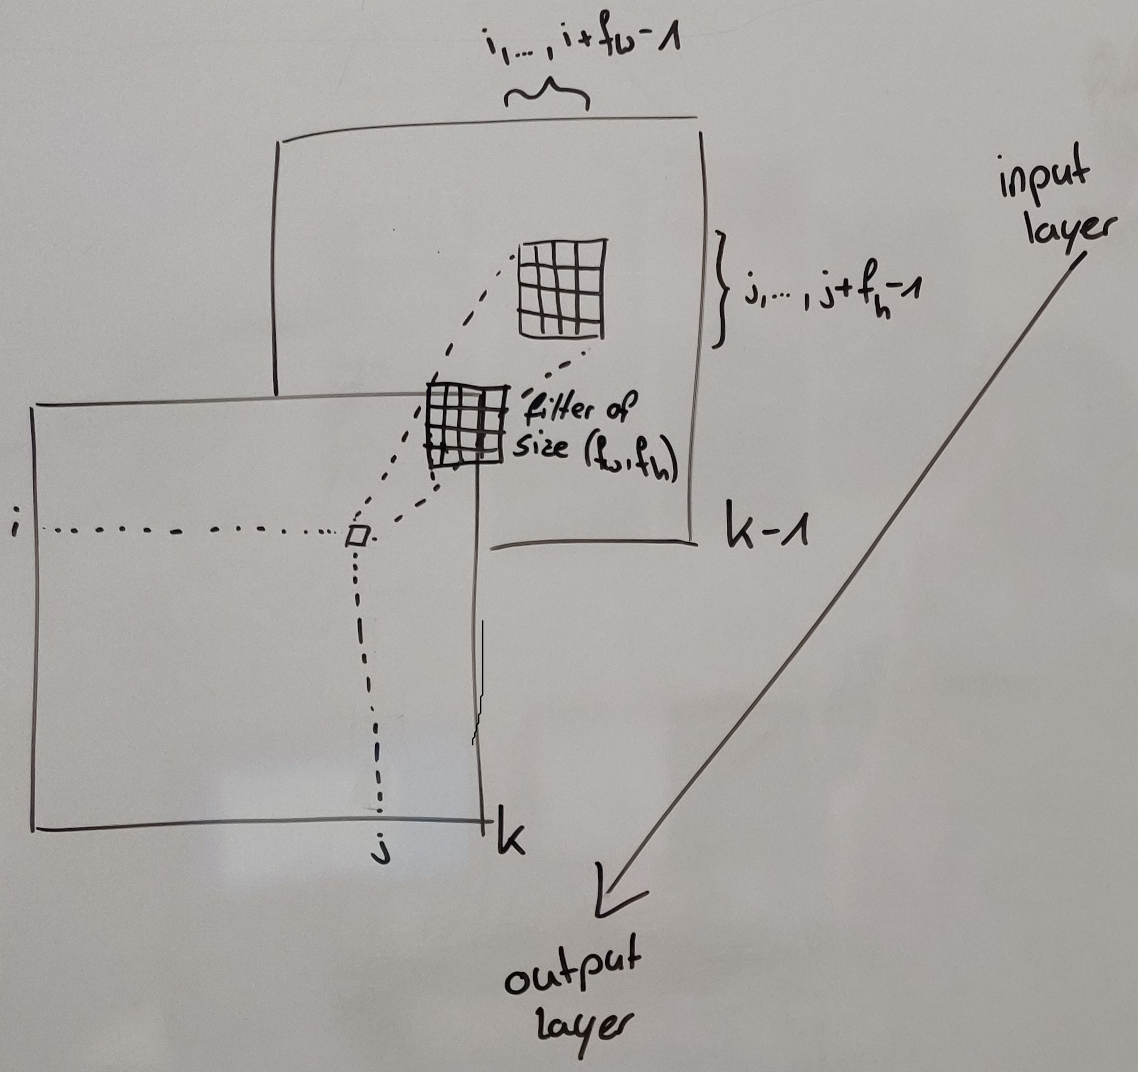
\includegraphics[width=0.8\textwidth]{images/convolution_template}
    \caption{Receptive field of a convolution operation}
    \label{fig:convolution}
\end{figure}

There are different ways to handle the edges of the grid. If no special action is taken, the output layer will be smaller in terms of edge length. For this reason \emph{zero padding} is often used to enlarge the input layer before convolution is performed. With an appropriate padding it is possible to preserve the width and height of the layer. Another parameter that affect the size of the output layer is called \emph{stride}, that controls the distance between to neighbouring receptive fields.~\cite[p.~361]{praxiseinstieg_ml17}

The trainable parameters in a convolution layer are the weights and biases used for the matrix multiplication introduced earlier. One specific set of weights and biases is called a \emph{filter}. It is responsible for detecting one single feature of the input layer. The output of a filter is thus referred to as \emph{feature map}. To inspect multiple features of the input, a convolution layer usually consists of multiple filters that are trained and calculated independently. In the end, the output of a convolution layer are multiple feature maps, each highlighting one single feature of the input.~\cite[p.~363f]{praxiseinstieg_ml17}

As stated by Goodfellow et al.\ in~\cite{DLbook16} the convolution operation has some properties that are highly valuable to build an efficient and powerful neural network:
\begin{enumerate}
    \item It leverages sparse interactions between the layers of a neural network.
    \item Many parameters are shared and reused throughout a whole layer.
    \item The operation is equivariant to translation of the input.
\end{enumerate}





\cite{DLbook16}
330: NN use only matrix multiplication. meaning every output unit of one layer interacts with the all input units of the next layer. convolution leverages sparse interactions. for example images can have millions of pixels, but to detect edges it is enough to only look at a few pixels at a time. thus we can have a kernel smaller than the image size resulting in fewer parameters. This reduces memory requirements of the model and increases statistical efficiency.

331, 333: another advantage is parameter sharing. with matrix multiplication you usually have a weight matrix, where each value is used only once. convolution operation uses parameter sharing, because one kernel is applied multiple times on the same image. and since kernel is smaller than image, it again reduces number of parameters by a significant amount.

334f: due to parameter sharing, convolution operation is equivariant to translation. Meaning, if you move parts of the input convolution will still give you the same output, just with the moved detection. This is especially helpful for working with images, as object might be in different locations of the image, but should still be realized.

\subsubsection{Pooling}
\cite{DLbook16}
335: Pooling replaces output of certain location with a summary of the nearby outputs. Max Pooling reports the maximum value inside a rectangular neighborhood. Other functions: (weighted) average or $L^2$ norm.


\begin{figure}[h]
    \centering
    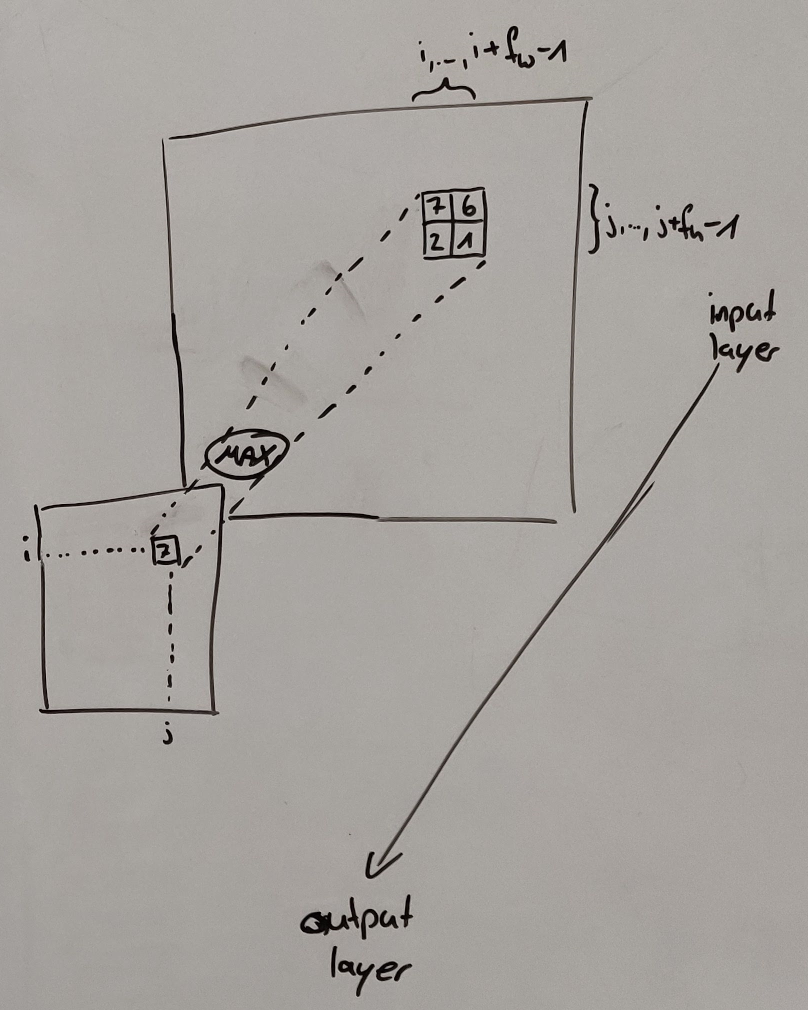
\includegraphics[width=0.8\textwidth]{images/maxpool}
    \caption{Max pooling \cite{stanford_convnet}}
    \label{fig:pooling}
\end{figure}

\cite{stanford_convnet}
Module 2: pooling layers between conv layers are common architecture. thereby you progressively reduce the spatial size and also number of params later in the net. pooling operates on all feature maps independently. For example pooling with kernel size 2x2 and stride 2 downsamples the input, so that 75\% of information is discarded.

Pooling layer are not trainable, because they compute a given function on the input elements. This function is oftentimes MAX function, also other variation like AVG oder L2-norm are used. However, pooling is configurable for the hyperparameters kernel size and stride.

\subsubsection{Others}
Batch Normalization, ReLU Activation, etc

\subsection{Reference Architectures}

\subsubsection{U-Net architecture}
\cite{unet15}
network architecture consists of a contracting path and an expansive path. contraction follows the typical architecture of convolutional network. repeated application of 3x3 convolutions, followed by ReLU and 2x2 max pooling. stride 2 for downsampling, features double for each contraction.
expansive path is upsampling followed by 2x2 convolution. also concatenation of the cropped feature map from the corresponding feature map from contraction path.
final layer is 1x1 convolution to map feature vector to desired number of classes. Demonstrated results with the EM segmentation challenge (\cite{isbi_challenge}), where they achieved very good results.

\begin{figure}[h]
    \centering
    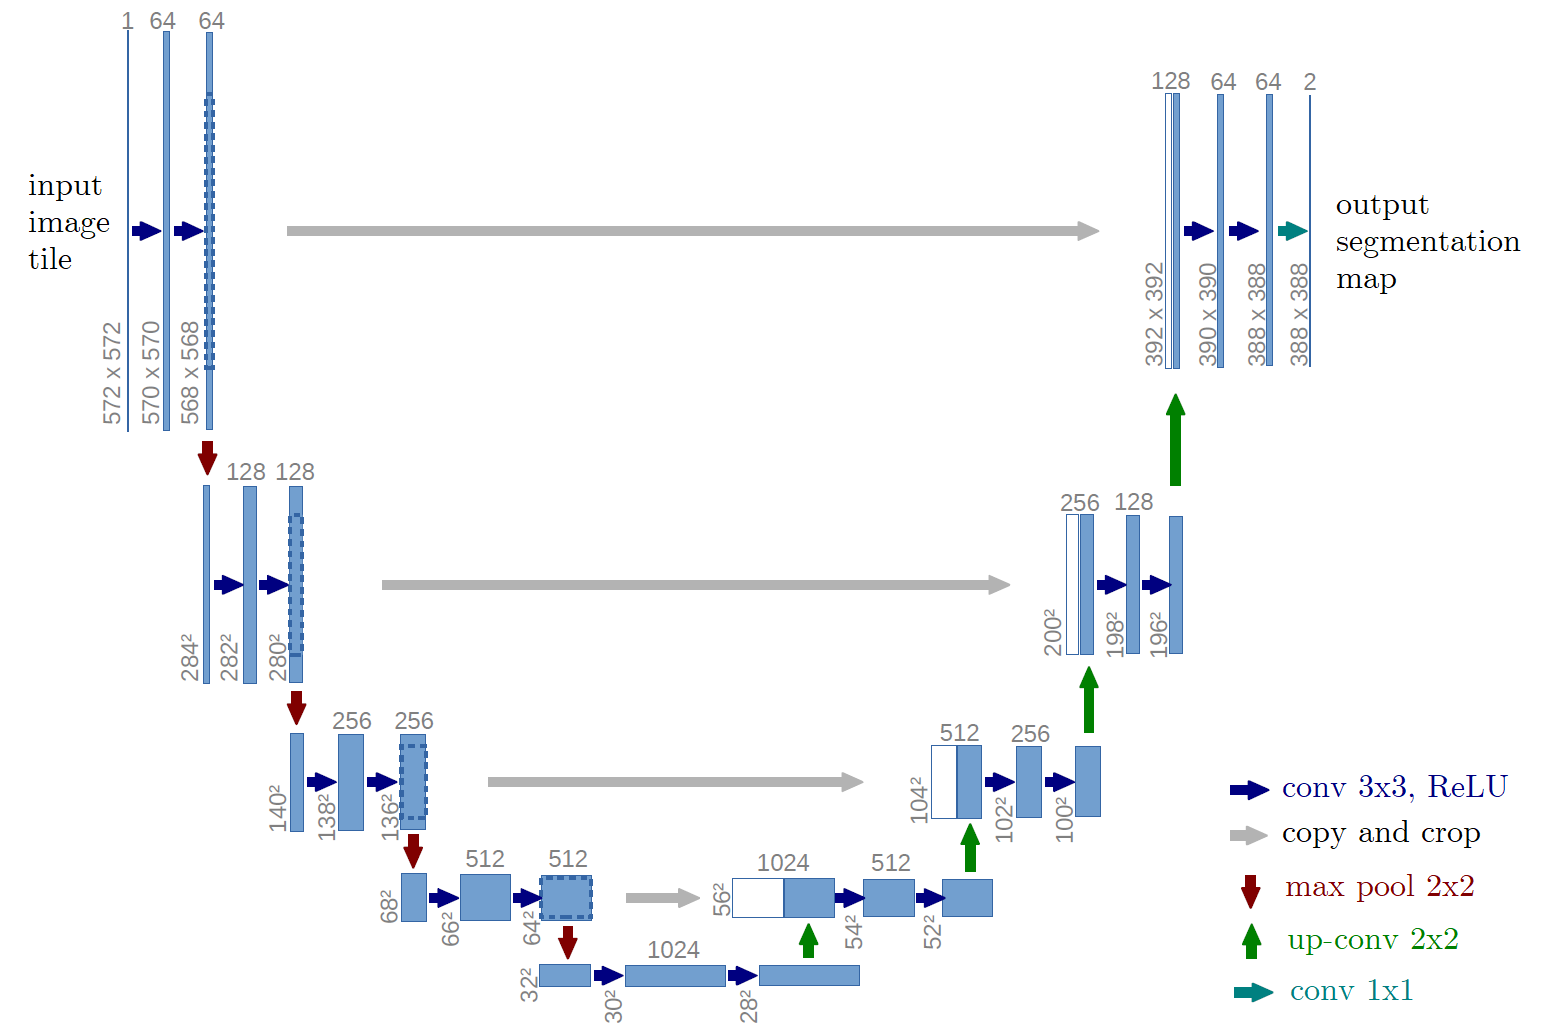
\includegraphics[width=0.9\textwidth]{images/u-net-architecture}
    \caption{U-Net Architecture \cite{unet15}}
    \label{fig:unet_architecture}
\end{figure}

\subsubsection{DenseNet Architecture}
\cite{densenet18}
NN architectures tended to get deeper and deeper. This brings problem of vanishing gradients because input data flows through so many layers. Different approaches to solve this. Authors of paper decided to connect all layers with matching feature map sizes. Features are combined by concatenation. This leads to many connections in a deep network, thus called Dense Convolutional Network (DenseNet).

Authors see layers as state of the network. For layer state to be accessible by next layers, the layer needs to pass the state. With their architecture, they differentiate between information coming from earlier layers and information being mined in the current layer. They keep layer narrow, each layer only adds small pieces of new information, existing information is not changed. All of that leads to having fewer parameters than traditional architectures.

Improved flow of gradients throughout the network. Every layer has access to original input signal and gradients from the loss function. Allows for even deeper architectures and prevents vanishing gradients. Make it easier to train the network.


\begin{figure}[h]
    \centering
    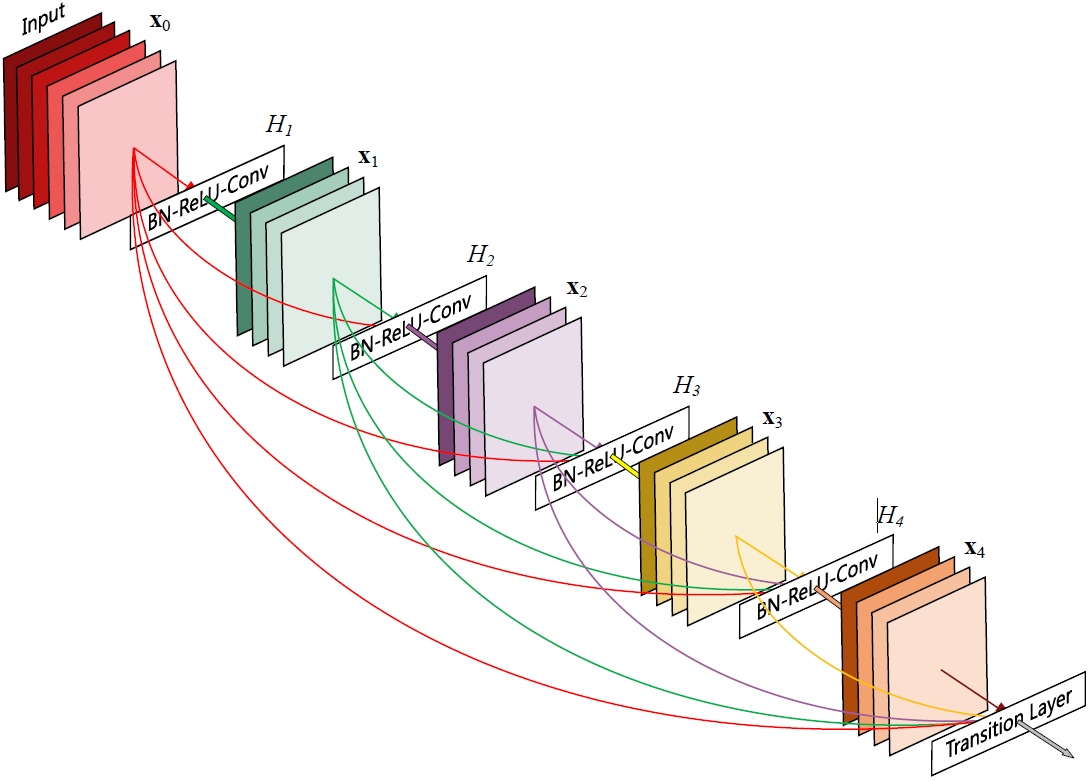
\includegraphics[width=0.9\textwidth]{images/dense-net-architecture}
    \caption{Densely Connected Convolutional Architecture \cite{densenet18}}
    \label{fig:densenet_architecture}
\end{figure}

\subsection{Architecture Comparison}
Interesting for architecture comparison: \cite{imseg_architecures}

\begin{itemize}
    \item point out the common characteristics and differences of the architectures
    \item compare use cases of the architectures and how they perform on them
\end{itemize}

\newpage